\documentclass[12pt,german]{article}
\usepackage{listings}
%\usepackage[utf8]{inputenc}
\usepackage{inputenc}
\usepackage{graphicx}

\lstset{
extendedchars=\true,
%inputencoding=utf8,
basicstyle=\ttfamily,
columns=fullflexible,
xleftmargin=5pt,
frame=single,
breaklines=true,
postbreak=\mbox{{$\hookrightarrow$}\space},
}


\begin{document}

\title{Übungsaufgaben I, SBV1 }
\author{Lisa Panholzer, Lukas Fiel}
\maketitle


\newpage
\section{Gauss Filter}
Es wurde ein Gauss Filter als ImageJ Filter implementiert. Die Behandlung der Randpixel wurde aus der Lehrveranstaltung übernommen. Gemeinsam mit dem Vortragenden Gerald Zwettler wurde die Java Klasse \textit{ConvolutionFilter} erweitert um auch die Randbereiche eines Bildes angemessen zu behandeln. In Heimarbeit wurde die Klasse um die Methode \textit{GetGaussMask} erweitert. In dieser wird die Verteilung einer Gauss Kurve auf eine 2 dimensionale Maske übertragen. \\

Anschlißend wurde eruiert welches Verhältnis von Sigma zum Radius der Maske eine klar zu erkennende Glocke darstellte. $ \frac{2}{4} $ hat die gewünschte Eigenschaft. 
\begin{table}[h]
  \centering
  \begin{tabular}{| c | c | c |}
    \hline
    $ \frac{sigma}{radius} $ & Masken Surface Plot & gefiltertes Bild \\
    \hline
    $ \frac{1}{4} $ &
	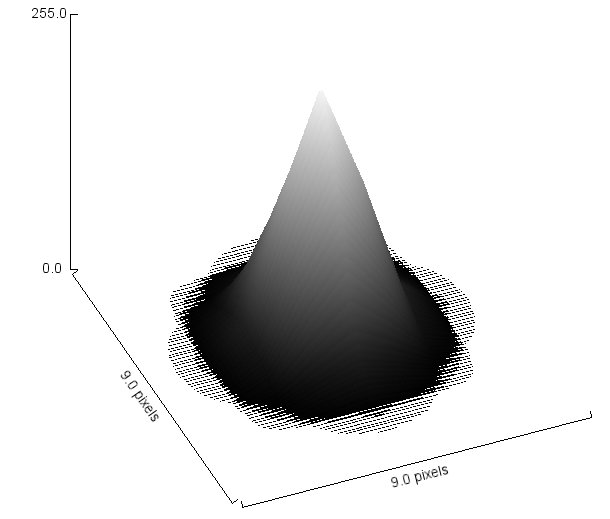
\includegraphics[width=4cm]{../testData/Gauss/GaussBellR4S1.jpg} & 	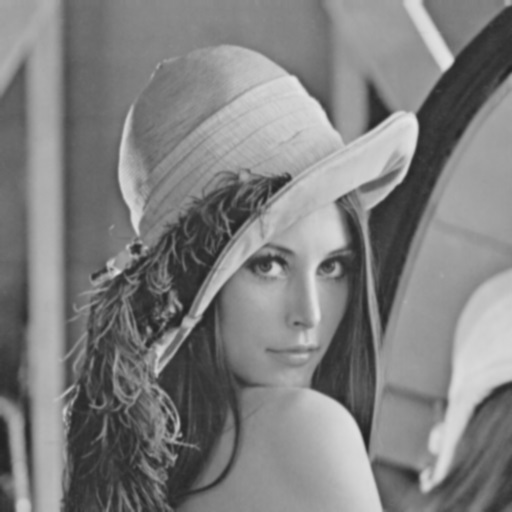
\includegraphics[width=4cm]{../testData/Gauss/LenaR4S1.jpg} \\
	    \hline
    $ \frac{2}{4} $ &
	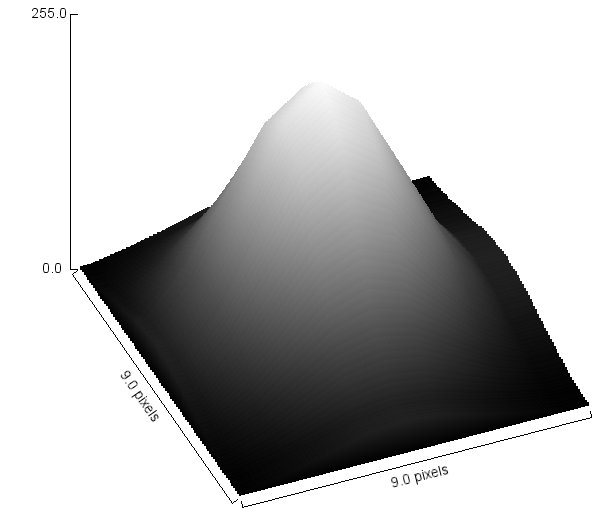
\includegraphics[width=4cm]{../testData/Gauss/GaussBellR4S2.jpg} & 	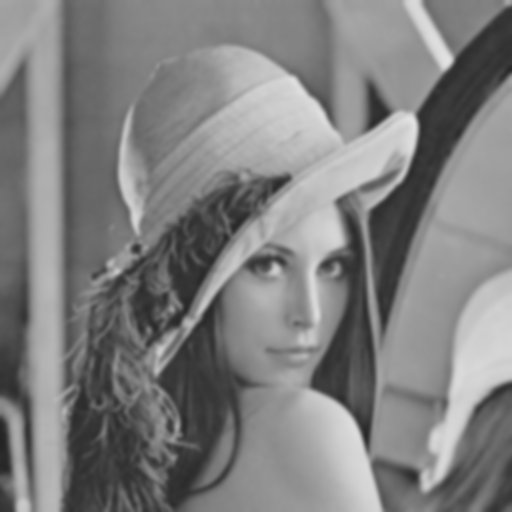
\includegraphics[width=4cm]{../testData/Gauss/LenaR4S2.jpg} \\
	    \hline
    $ \frac{3}{4} $ &
	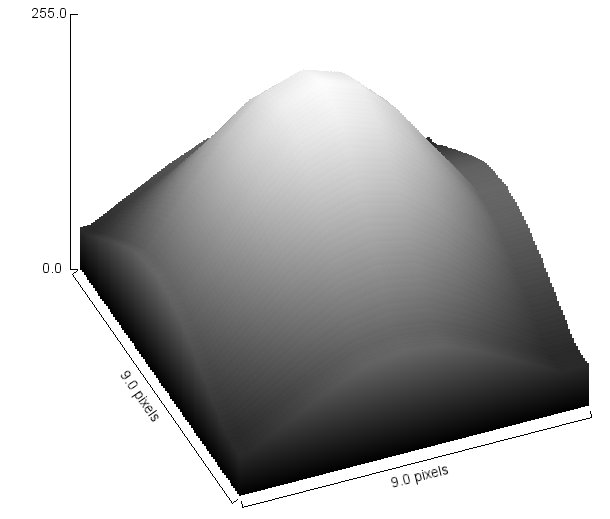
\includegraphics[width=4cm]{../testData/Gauss/GaussBellR4S3.jpg} & 	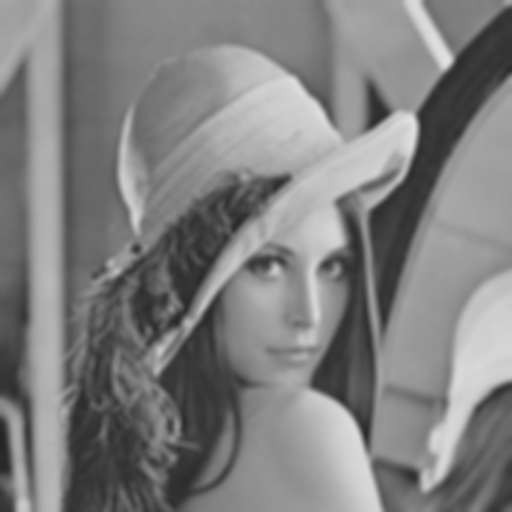
\includegraphics[width=4cm]{../testData/Gauss/LenaR4S3.jpg} \\
	    \hline
    $ \frac{4}{4} $ &
	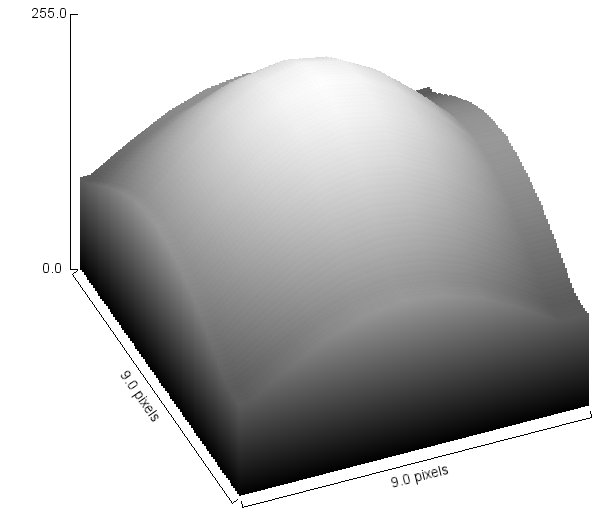
\includegraphics[width=4cm]{../testData/Gauss/GaussBellR4S4.jpg} & 	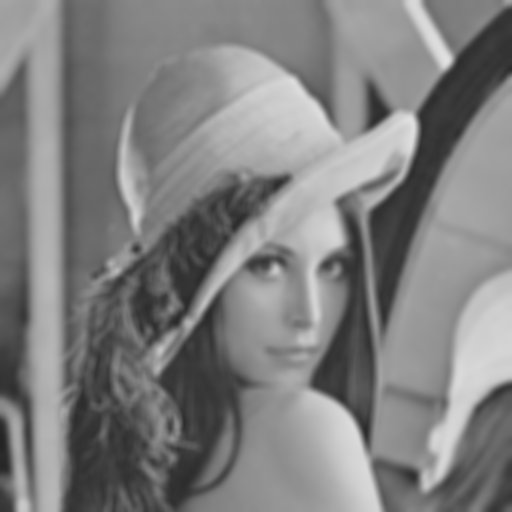
\includegraphics[width=4cm]{../testData/Gauss/LenaR4S4.jpg} \\
  \end{tabular}
  \caption{Gauss Filter Größen}
  \label{tab:GaussFilterGroessen}
\end{table}

Weiters wurde der Übergang von scharfen Kanten und Verläufen mit dem Gauss Filter gefiltert. Man bemerkt gut, dass bei einem Intensitätsverlauf kaum ein Filtereffeckt sichtbar ist, während Kanten deutlich verschwommen erscheinen. Gewähltes Verhältnis: $ \frac{sigma}{radius} = \frac{2}{4} $
\begin{table}[h]
  \centering
  \begin{tabular}{| c | c | c |}
    \hline
    $ \frac{sigma}{radius} $ & Masken Surface Plot & gefiltertes Bild \\
    \hline
    $ \frac{1}{4} $ &
	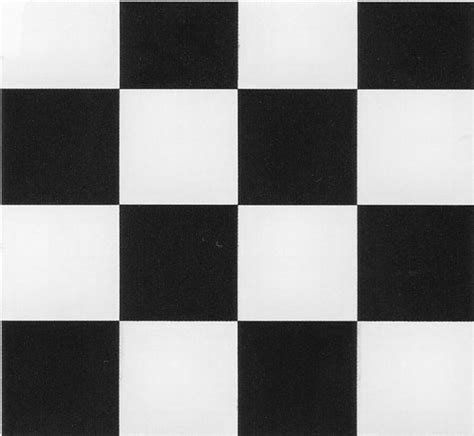
\includegraphics[width=4cm]{../testData/Gauss/Schachbrett.jpg} & 	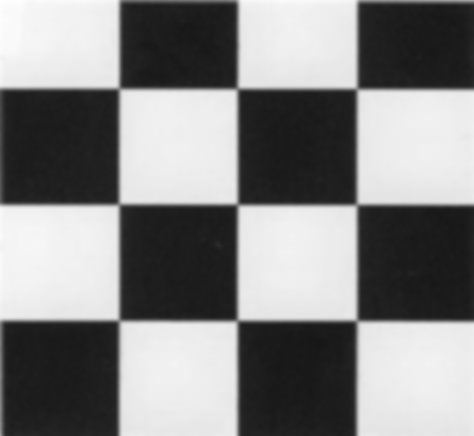
\includegraphics[width=4cm]{../testData/Gauss/SchachbrettR4S2.jpg} \\
	    \hline
    $ \frac{2}{4} $ &
	
\includegraphics[width=4cm]{../testData/Gauss/Regenbogen.jpg} & 	
\includegraphics[width=4cm]{../testData/Gauss/RegenbogenR4S2.jpg} \\
  \end{tabular}
  \caption{Gauss Filter Evaluierung}
  \label{tab:GaussFilterEvaluierung}
\end{table}

\subsubsection{Code}
\lstinputlisting[frame=single,language=JAVA,breaklines=true]{../Gauss_.java}
\lstinputlisting[frame=single,language=JAVA,breaklines=true]{../ConvolutionFilter.java}



%% -------------------------------------------------------------------------------------------------------------------------
%% ------------------------------------------- ZWEITES BEISPIEL -----------------------------------------------------
%% -------------------------------------------------------------------------------------------------------------------------
\newpage
\section{MedianFilter}
Der MedianFilter kann leider nicht mittels der Klasse \textit{ConvolutionFilter} implementiert werden, da die Maske für dieses Vorgehen konstant sein müsste. Das Prinzip ist allerdings sehr ähnlich. Es wird ein Pixel in Mitten einer quadratischen Umgebung betrachtet. Dieses Pixel soll im resultierenden Bild als der Median Wert der Umgebung gesetzt werden. \\
Implementiert wurde dies durch das Herausschneiden der interessanten Umgebung aus einer Kopie des Ursprungsbildes und anschließender Medianwertberechnung. 
\subsubsection{Code}
\lstinputlisting[frame=single,language=JAVA,breaklines=true]{../Median_.java}
\subsubsection{resultierendes Bild}
\begin{figure}[h]
	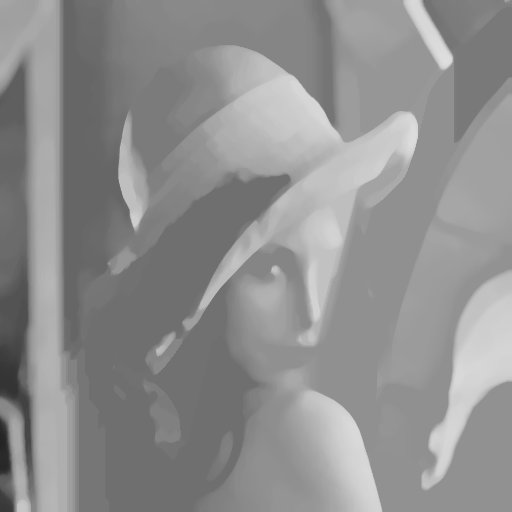
\includegraphics[width=7cm]{../testData/Results/median.jpg}
\end{figure}



%% -------------------------------------------------------------------------------------------------------------------------
%% ------------------------------------------- DRITTES BEISPIEL -----------------------------------------------------
%% -------------------------------------------------------------------------------------------------------------------------
\newpage
\section{Steuerung des Filtereffekts }
\subsection{Code}
\lstinputlisting[frame=single,language=JAVA,breaklines=true]{../FiltereffektEvaluierung_.java}
\subsubsection{Ablaufund Idee}
\begin{figure}[h]
	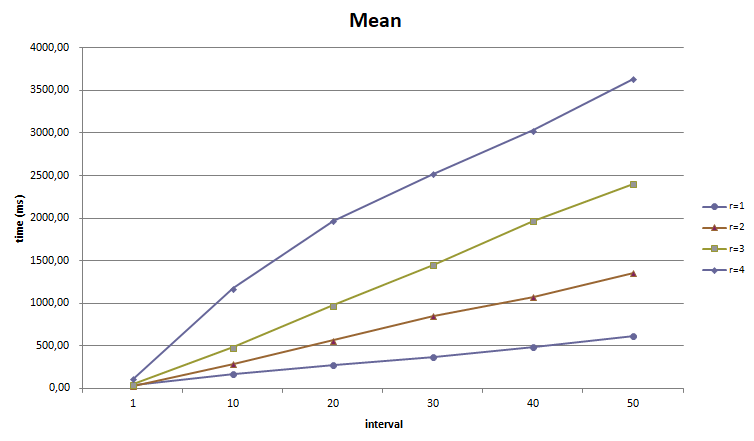
\includegraphics[width=7cm]{TimeEvaluationGraph_Mean.png}
\end{figure}
\begin{figure}[h]
	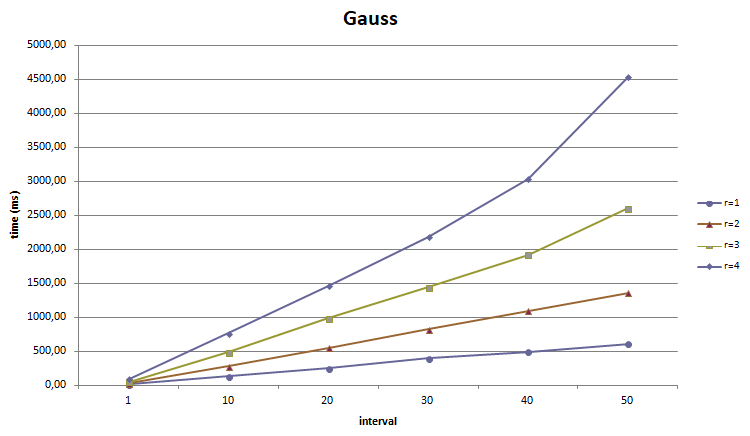
\includegraphics[width=7cm]{TimeEvaluationGraph_Gauss.png}
\end{figure}
\begin{figure}[h]
	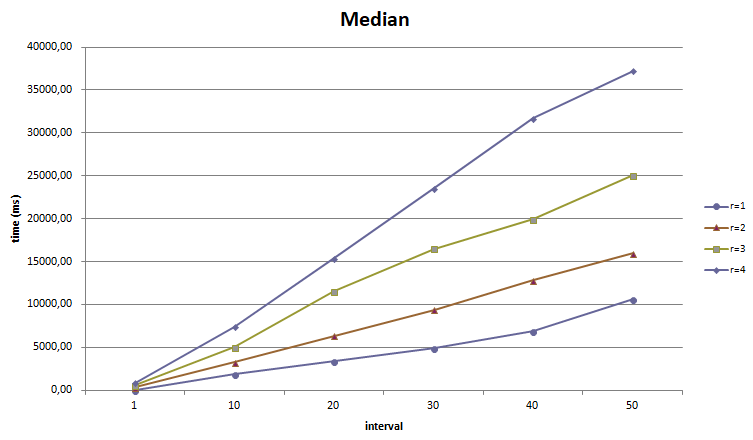
\includegraphics[width=7cm]{TimeEvaluationGraph_Median.png}
\end{figure}

\subsubsection{Tests}

%% -------------------------------------------------------------------------------------------------------------------------
%% ------------------------------------------- VIERTES BEISPIEL -----------------------------------------------------
%% -------------------------------------------------------------------------------------------------------------------------
\newpage
\section{Histogrammeinebnung  }
\subsection{Code}
\lstinputlisting[frame=single,language=JAVA,breaklines=true]{../Median_.java}
\subsection{Tests}


%% -------------------------------------------------------------------------------------------------------------------------
%% ------------------------------------------- FÜNFTES BEISPIEL -----------------------------------------------------
%% -------------------------------------------------------------------------------------------------------------------------
\newpage
\section{ Raster-Entfernung im Frequenzraum}
\subsection{Workflow}
\begin{itemize}
	\item Starten von \textit{imageJ.exe}
	\item Öffnen eines Bildes
	\item \textit{Process $\rightarrow$ FFT $\rightarrow$ FFT}
	\item Zuschneiden des interessanten Bereichs im FFT Bild
	\item \textit{Process $\rightarrow$ FFT $\rightarrow$ inverse FFT}
\end{itemize}

\subsection{Beispiele}

\subsubsection{Auge}
Es wurde ein Bild gewählt, welches (wie bei einem Plakatdruck) Punkte in regelmässigen Abständen aufweist. Die eigentliche Bildinformation steckt in der Dicke er Punkte. Eine FFT Transformation zeigt deutlich ein periodisches Muster. Will man nur die eigentliche Bildinformation gewinnen, müssen hochfrequente Anteile des Bildes entfernt werden. Tabelle \ref{tab:AuswertungAuge} zeigt deutlich dass durch ein Entfernen der Randbereiche (höhere Frequenzen) im FFT Bild und die anschließende Rücktransformation die eigentliche Bildinformation gewonnen werden konnte.
\begin{table}[h]
  \centering
  \begin{tabular}{c | c}
    \hline
    Bild & FFT \\
    \hline
	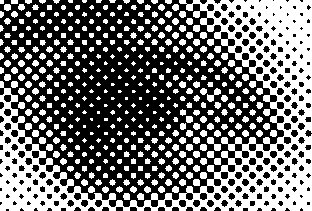
\includegraphics[width=4cm]{../testData/Auge.jpg} & 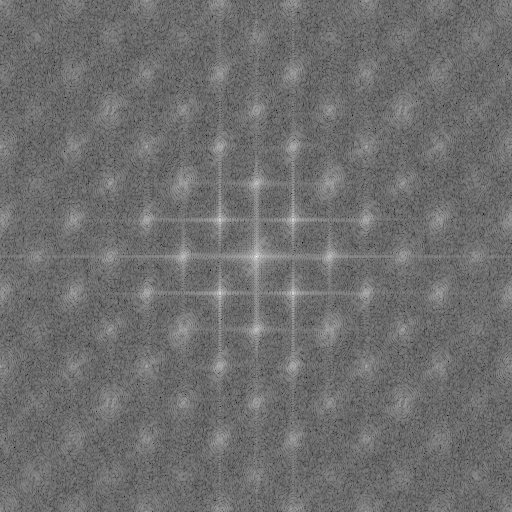
\includegraphics[width=4cm]{../testData/Results/Auge/FFT_of_Auge.jpg} \\
    \hline
    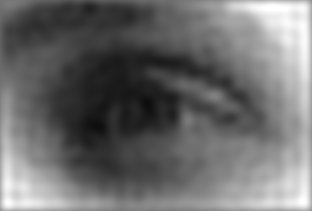
\includegraphics[width=4cm]{../testData/Results/Auge/reduced_Auge.jpg} & 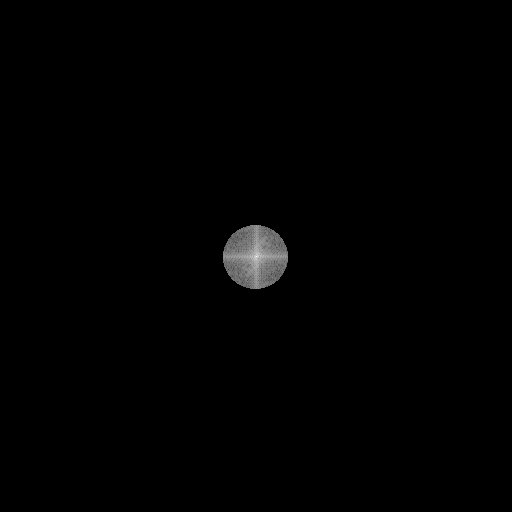
\includegraphics[width=4cm]{../testData/Results/Auge/reduced_FFT_of_Auge.jpg} \\
  \end{tabular}
  \caption{Auswertung Auge}
  \label{tab:AuswertungAuge}
\end{table}


\subsubsection{Elefant}
In diesem Bild sind viele periodisch auftretende Elemente enthalten. Es wurde versucht die Schrift, die Gitterstäbe im Hintergrund und natürlich die beiden Tiere gut sichtbar zu erhalten. Da aber die Gitterstäbe selbst periodisch im Bild vorkommen und auch die Schrift sich wiederholende senkrechte Kanten hat, war dies nicht einfach. Ein Auslöschen der horizontalen und vertikalen Anteile aus dem Bild brachte in unseren Versuchen das beste Ergebnis. Hierbei ist aber zu beachten, dass das Zentrum des FFT Bildes die meiste Information enthält. Daher wurde diese bestehen gelassen. Auch die Randbereiche der FFT wurden belassen, da diese für scharfe Kanten im Bild verantwortlich sind. Ein Wegschneiden dieser Bereiche würde auch die Konturen des Elefanten und die Schrift unscharf machen.
\begin{table}
  \centering
  \begin{tabular}{c | c}
    \hline
    Bild & FFT \\
    \hline
	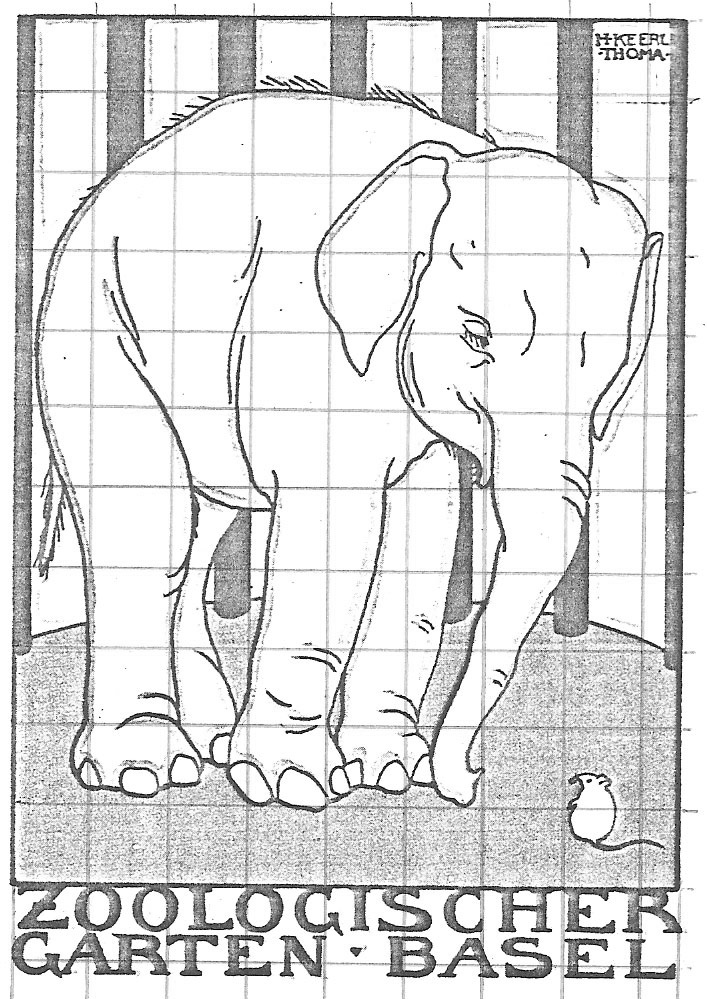
\includegraphics[width=4cm]{../testData/Elefant.jpg} & 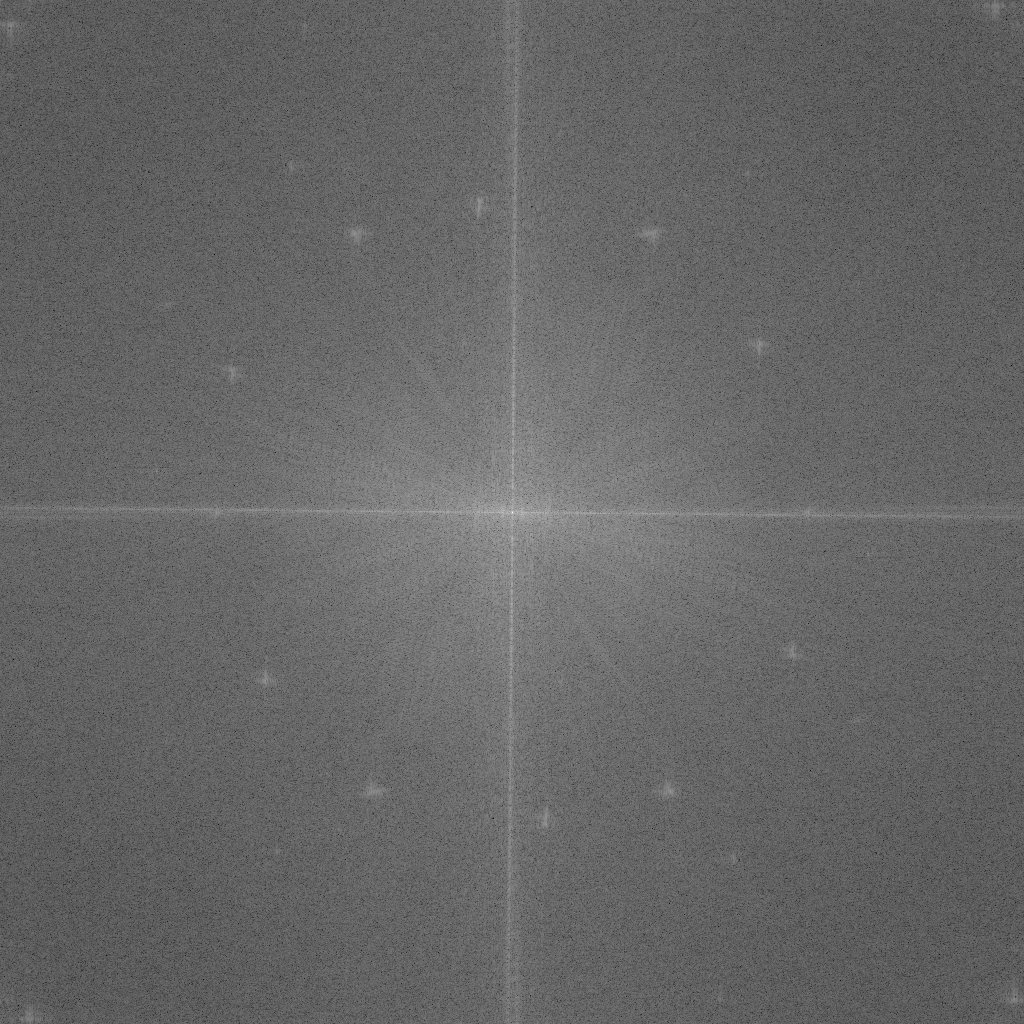
\includegraphics[width=4cm]{../testData/Results/Elefant/FFT_of_Elefant.jpg} \\
    \hline
    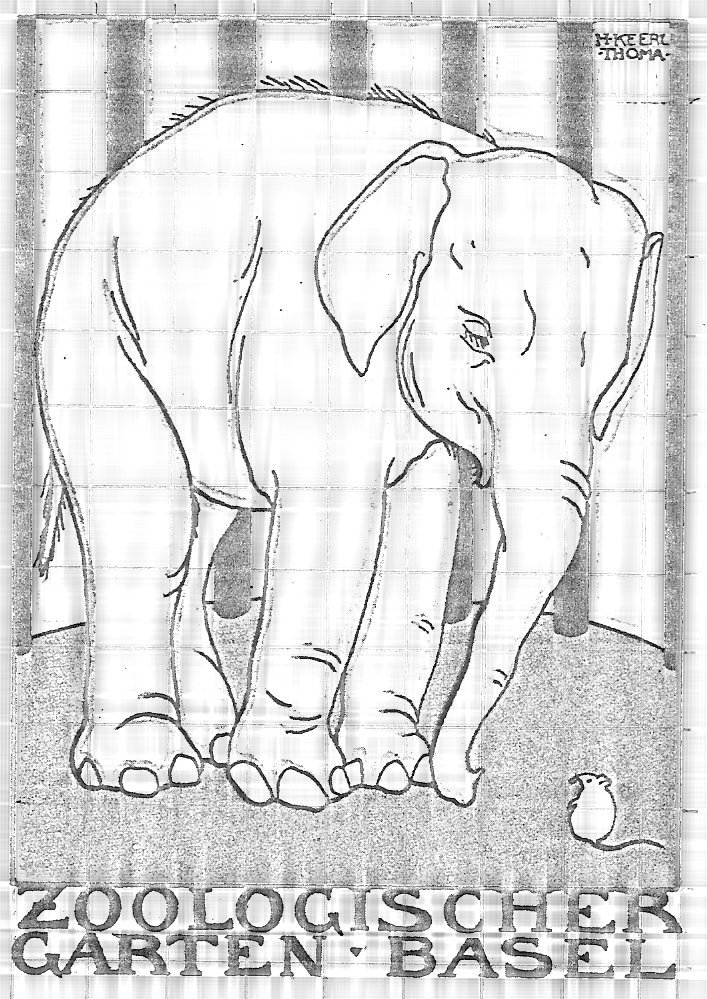
\includegraphics[width=4cm]{../testData/Results/Elefant/reducedElefant.jpg} & 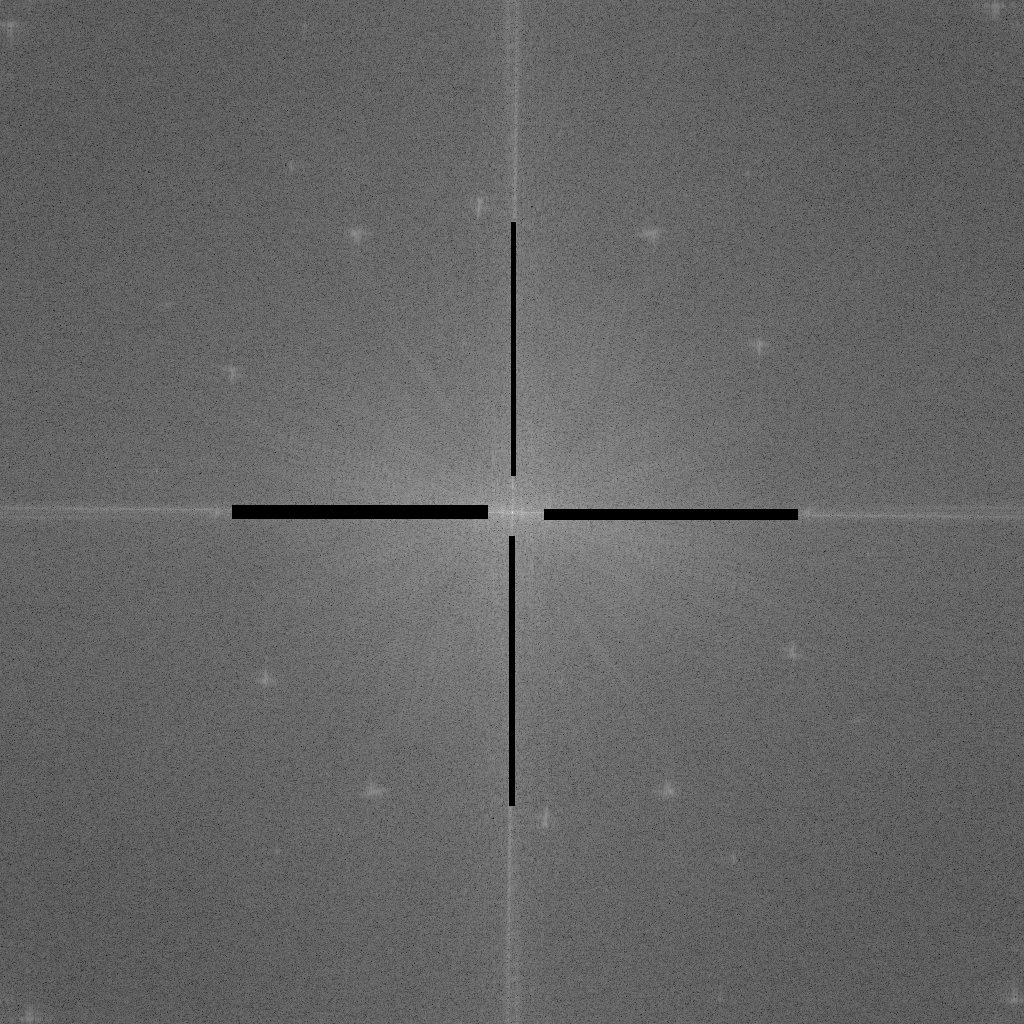
\includegraphics[width=4cm]{../testData/Results/Elefant/reducedFFT_of_Elefant.jpg} \\
  \end{tabular}
  \caption{Auswertung Elefant}
  \label{tab: AuswertungElefant }
\end{table}

\subsubsection{Lochgitter}
Hier handelt es sich um ein perspektivisch beläuchtetes Lochgitter. Die Löcher sind sechseckig. In der FFT erkennt man gut die Periodizität. Ein Wegschneiden der äusseren Bereiche der FFT und eine Rücktransformation zeigt deutlich die perspektivische Beläuchtung. Das Lochgitter konnte aber vollkommen entfernt werden. Interessant ist auch zu bemerken, dass im Rücktransformierten Bild eine Schrift \textit{"colourbox"} deutlich zu erkennen ist. Bei genauerer Betrachtung des Ursprungsbildes ist diese hinter dem Gitter zu erkennen.  
\begin{table}
  \centering
  \begin{tabular}{c | c}
    \hline
    Bild & FFT \\
    \hline
	
\includegraphics[width=4cm]{../testData/Lochgitter.jpg} & 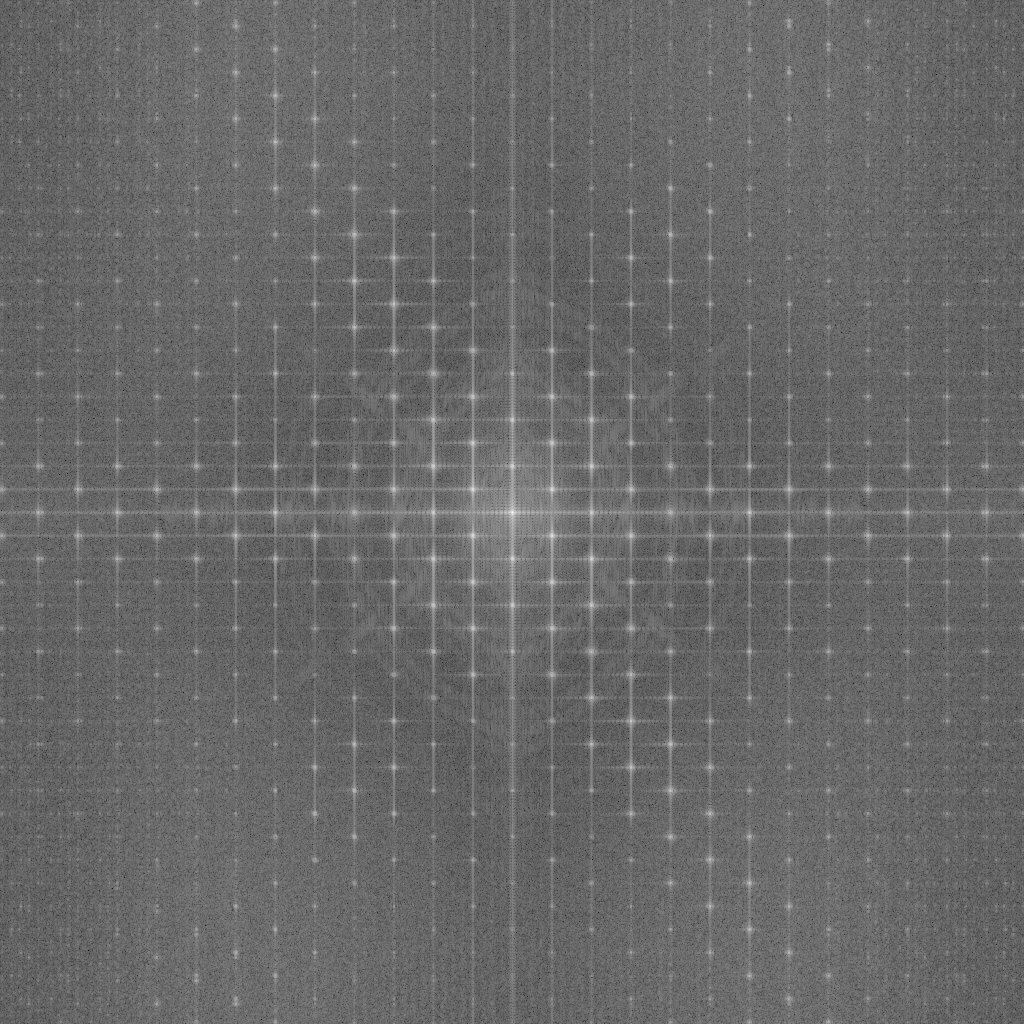
\includegraphics[width=4cm]{../testData/Results/Lochgitter/FFT_of_Lochgitter.jpg} \\
    \hline
    
\includegraphics[width=4cm]{../testData/Results/Lochgitter/reducedLochgitter.jpg} & 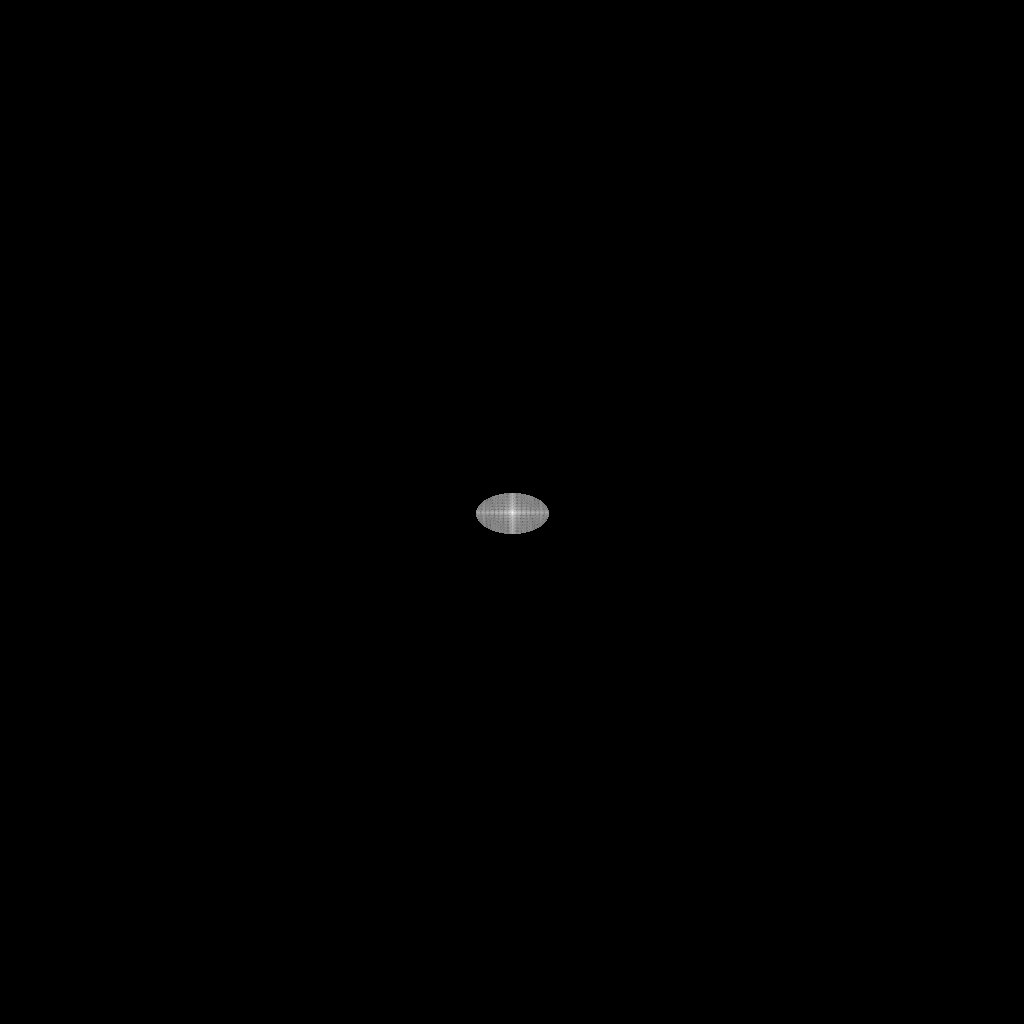
\includegraphics[width=4cm]{../testData/Results/Lochgitter/reducedFFT_of_Lochgitter.jpg} \\
  \end{tabular}
  \caption{Auswertung Lochgitter}
  \label{tab:AuswertungLochgitter}
\end{table}

\subsection{Analyse eines Frequenzmusters}
Ein sich wiederholendes Muster in einem Bild ist mittels \textit{FFT} gut vom eigentlichen Bildinhalt zu unterscheiden. So kann das Muster entfernt werden und das eigentliche Bild mittels \textit{inverseFFT} ermittelt werden. Leider sind reale Bilder meist nicht genau horizontal ausgerichtet. Auch kann man nicht davon ausgehen, dass sich wiederholende Elemente in der Realität unverzerrt in einem Bild dargestellt sind. Kanten werden nur in den seltensten Fällen genau durch einen Pixel des Bildes dargestellt. All diese Umstände machen es schwer aus einem Alltagsfoto wiederkehrende Elemente herauszufiltern.

\section{Anhang}
\lstinputlisting[frame=single,language=JAVA,breaklines=true]{../ConvolutionFilter.java}


\end{document}
